\documentclass[aspectratio=169]{beamer}
\renewcommand{\rmdefault}{cmr}
\usepackage{helvet}
\renewcommand{\ttdefault}{cmtt}
\usepackage[T1]{fontenc}
\usepackage[utf8]{inputenc}
\setcounter{secnumdepth}{3}
\setcounter{tocdepth}{3}
\usepackage{amsbsy}
\usepackage{amstext}
\usepackage{amssymb}
\usepackage{graphicx}
\usepackage{hyperref}
\usepackage[english]{babel}
\hypersetup{unicode=true,breaklinks=false,pdfborder={0 0 0},pdfborderstyle={},colorlinks=true,linkcolor=blue, citecolor=blue, urlcolor=blue}

\makeatletter
%%%%%%%%%%%%%%%%%%%%%%%%%%%%%% Textclass specific LaTeX commands.
% this default might be overridden by plain title style
\newcommand\makebeamertitle{\frame{\maketitle}}%
% (ERT) argument for the TOC
\AtBeginDocument{%
  \let\origtableofcontents=\tableofcontents
  \def\tableofcontents{\@ifnextchar[{\origtableofcontents}{\gobbletableofcontents}}
  \def\gobbletableofcontents#1{\origtableofcontents}
}

%%%%%%%%%%%%%%%%%%%%%%%%%%%%%% User specified LaTeX commands.
\usepackage{ifthen}
\usepackage{multirow,bigstrut}
\usepackage{tikz}
\usetikzlibrary{patterns,decorations.pathreplacing,shapes}
\usetikzlibrary{arrows}
\usepackage{rotating}
\usepackage{pdflscape}
\usepackage{makecell}
\usepackage{graphicx}
\usepackage{booktabs}

\defbeamertemplate*{footline}{guildford foot theme}
{
  \leavevmode%
  \hbox{%
  \begin{beamercolorbox}[wd=.7\paperwidth,ht=1cm,dp=0ex,left]{}%
    {
    \insertsectionnavigationhorizontal{.5\paperwidth}{}{}
    }
 \end{beamercolorbox}
 \begin{beamercolorbox}[wd=0.31\paperwidth,ht=1cm,dp=0ex,right]{}%
{\tiny
\insertframenumber{} / \inserttotalframenumber\hspace*{5ex}
}
 \end{beamercolorbox}}%
  \vskip5pt%
}

\beamertemplatenavigationsymbolsempty
\usefonttheme{professionalfonts}
\usecolortheme[RGB={0,0,125}]{structure}
\setbeamersize{text margin left=10px}
\definecolor{newblue}{rgb}{0,0,0.6}
\setbeamercolor{alerted text}{fg=newblue}
\setbeamertemplate{frametitle}[default][center]

\RequirePackage{ifthen}

\newboolean{sectiontoc}
\setboolean{sectiontoc}{true}

\AtBeginSubsection[]
{
  \ifthenelse{\boolean{sectiontoc}}{
  \begin{frame}[plain]
    \frametitle{Outline}
    \tableofcontents[sectionstyle=show/hide,subsectionstyle=show/shaded/hide]
  \end{frame}
}
}

\AtBeginSection[]
{
  \ifthenelse{\boolean{sectiontoc}}{
  \begin{frame}[noframenumbering,plain]
    \frametitle{Outline}
    \tableofcontents[sectionstyle=show/shaded,subsectionstyle=show/hide/hide]
  \end{frame}
}
}

\newcommand{\toclesssection}[1]{
   \setboolean{sectiontoc}{false}
   \section{#1}
   \setboolean{sectiontoc}{true}
}

\newcommand{\toclesssubsection}[1]{
   \setboolean{sectiontoc}{false}
   \subsection{#1}
   \setboolean{sectiontoc}{true}
}

\makeatother

\begin{document}

\title{\textit{UN3902: Economics of Public Policy Seminar} \\ Week 7: Taxation (in the US)}
\author{Michael Carlos Best}
\date{March 3, 2026}

\makebeamertitle

\section{Types of Taxation}

\begin{frame}
\frametitle{Types of Taxation: Taxes on Earnings and Income}
\begin{itemize}
  \setlength{\itemsep}{15pt} % Increase space
  \item \textbf{Payroll tax}: A tax levied on income earned on one's job.
  \item \textbf{Individual income tax}: A tax paid on individual income accrued during the year.
  \item \textbf{Capital gains}: Earnings from selling capital assets, such as stocks, paintings, and houses.
  \item \textbf{Corporate income tax}: Tax levied on the earnings of corporations.
\end{itemize}
\end{frame}

\begin{frame}
\frametitle{Types of Taxation: Taxes on Wealth}
\begin{itemize}
  \setlength{\itemsep}{15pt} % Increase space
  \item \textbf{Wealth taxes}: Taxes paid on the value of the assets, such as real estate or stocks, held by a person or family.
  \item \textbf{Property taxes}: A form of wealth tax based on the value of real estate, including the value of real estate.
  \item \textbf{Estate taxes}: A form of wealth tax based on the value of the estate left behind when one dies.
\end{itemize}
\end{frame}

\begin{frame}
\frametitle{Taxes on Consumption}
\begin{itemize}
  \setlength{\itemsep}{15pt} % Increase space
  \item \textbf{Sales taxes}: Taxes paid by consumers to vendors at the point of sale.
  \item \textbf{Excise tax}: A tax paid on the sales of particular goods, such as cigarettes or gasoline.
\end{itemize}
\end{frame}

\begin{frame}
\frametitle{Tax Revenues by Type of Tax in the United States}
\begin{itemize}
  \item The federal government receives a large portion of its tax revenue from individual income tax and payroll taxes.
  \item The two major sources of revenues for state and local governments are sales taxes and local property taxes.
\end{itemize}
\begin{center}
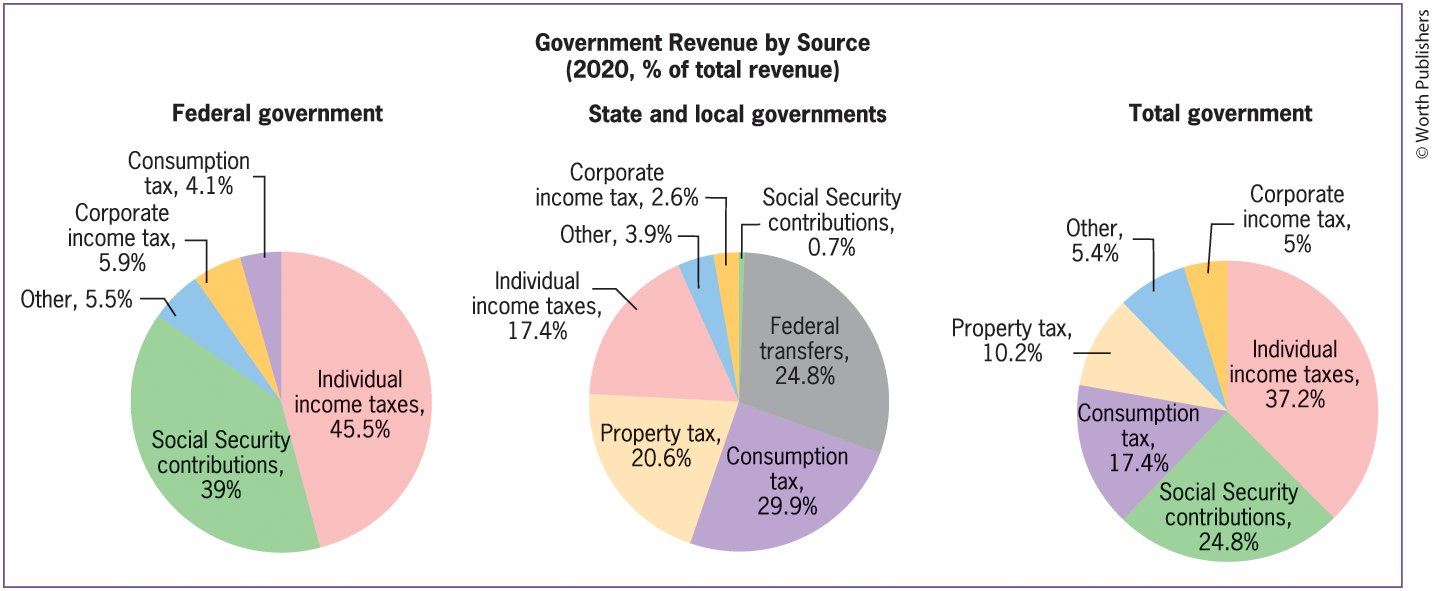
\includegraphics[width=0.95\textwidth]{images/figure_4_3.png}
\end{center}
\end{frame}

\begin{frame}
\frametitle{International Tax Revenues by Type of Tax}
\begin{itemize}
  \item Consumption taxes provide a greater portion of national government revenue in all OECD countries than in the United States.
\end{itemize}
\begin{center}
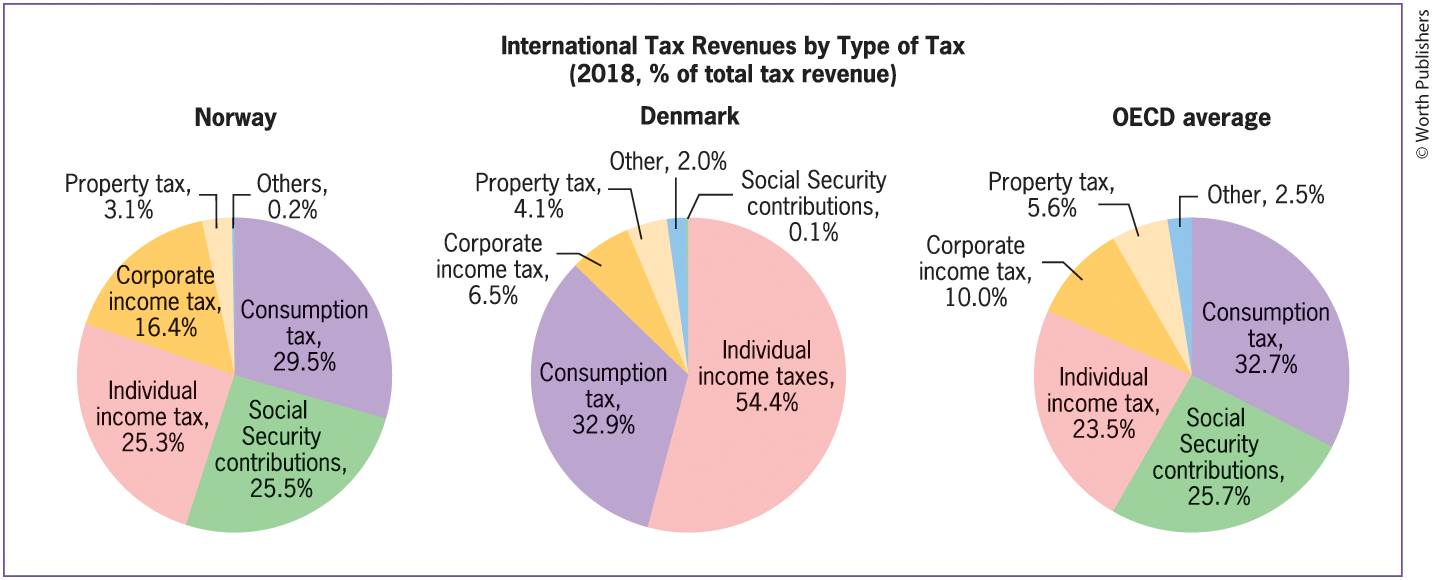
\includegraphics[width=0.95\textwidth]{images/figure_5_3.png}
\end{center}
\end{frame}

\section{Individual Income Tax Structure}

\begin{frame}
\frametitle{Structure of the Individual Income Tax: Computing the Tax Base}
\begin{itemize}
  \item Income tax is assessed on adjusted gross income minus deductions and exemptions.
  \item \textbf{Gross income}: The total of an individual's various sources of income.
  \item \textbf{Adjusted gross income (AGI)}: An individual's gross income minus certain deductions, such as contributions to IRAs.
  \item \textbf{Taxable income}: The amount of income left after subtracting exemptions and deductions from adjusted gross income.
\end{itemize}
\end{frame}

\begin{frame}
\frametitle{Individual Income Tax: Computing the Tax Base 1}
\begin{itemize}
  \item Adjustments vary over time but currently include:
\end{itemize}
\begin{enumerate}
  \item Some contributions to retirement savings.
  \item Alimony paid to a former spouse.
  \item Health insurance premiums paid by the self-employed.
  \item One-half the payroll taxes paid by the self-employed.
  \item Educator expenses and interest paid on student loans.
  \item Contributions to Health Savings Accounts.
  \item Expenses for job-related moves.
  \item Interest paid on student loans.
\end{enumerate}
\end{frame}

\begin{frame}
\frametitle{Individual Income Tax: Computing the Tax Base 2}
\begin{itemize}
  \item To form AGI from gross income, subtract exemptions and deductions.
  \item \textbf{Exemption}: A fixed amount a taxpayer can subtract from AGI for dependent member of a household as well as for the taxpayer and the taxpayer's spouse.
  \item Taxpayers can take one of two kinds of deductions:
\end{itemize}
\begin{enumerate}
    \item \textbf{Standard deduction}: A fixed amount that a taxpayer can deduct from taxable income.
    \item \textbf{Itemized deductions}: Alternative to the standard deduction whereby a taxpayer deducts the total amount of money spent on various expenses, such as gifts to charity and interest on home mortgages, medical expenses exceeding 10\% of AGI\ldots
  \end{enumerate}
\end{frame}

\begin{frame}
\frametitle{Tax Rates and Taxes Paid}
\begin{itemize}
  \item \textbf{Tax credits}: Amounts by which taxpayers are allowed to reduce the taxes they owe to the government through spending, for example, on child care.
  \item \textbf{Withholding}: The subtraction of estimated taxes owed directly from a worker's earnings.
  \item \textbf{Refund}: The difference between the amount withheld from a worker's earnings and the taxes owed if the former is higher.
\end{itemize}
\end{frame}

\begin{frame}
\frametitle{U.S. Federal Income Tax Rate Schedule, 2020}
\begin{center}
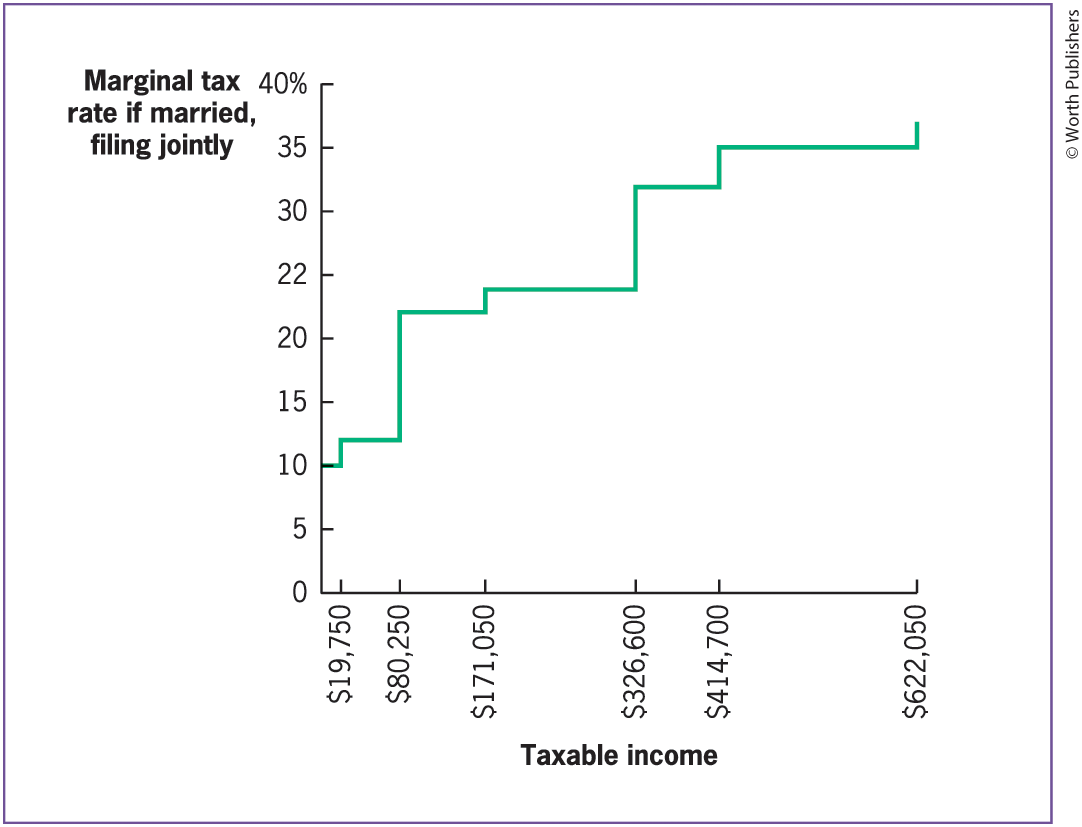
\includegraphics[height=\textheight]{images/figure_11_3.png}
\end{center}
\end{frame}

\section{Tax Design}

\subsection{Fairness and Equity}

\begin{frame}
\frametitle{Measuring the Fairness of Tax Systems}
\begin{itemize}
  \item Fairness is an important concern and elusive goal.
  \item Two key features of any tax system:
  \begin{itemize}
    \item \textbf{Marginal tax rate}: The percentage that is paid in taxes of the next dollar earned.
    \item \textbf{Average tax rate}: The percentage of gross income that is paid in taxes.
  \end{itemize}
  \item In the United States, the marginal tax rate rises with income, from 10\% to 37\%.
  \item Two distributional goals are considered in measuring tax fairness:
  \begin{itemize}
    \item \textbf{Vertical equity}: The principle that groups with more resources should pay higher taxes than groups with fewer resources.
    \item \textbf{Horizontal equity}: The principle that similar individuals who make different economic choices should be treated similarly by the tax system.
  \end{itemize}
\end{itemize}
\end{frame}

\begin{frame}
\frametitle{Measuring Vertical Equity}
\begin{itemize}
  \item Vertical equity likely requires progressive taxation.
  \item \textbf{Progressive}: Tax systems in which effective average tax rates rise with income.
  \item \textbf{Proportional}: Tax systems in which effective average tax rates do not change with income so that all taxpayers pay the same proportion of their income in taxes.
  \item \textbf{Regressive}: Tax systems in which effective average tax rates fall with income.
\end{itemize}
\end{frame}

\subsection{Taxation and Economic Efficiency}

\begin{frame}
\frametitle{Behavioral Responses to Taxation}
\begin{itemize}
  \item Arnold Harberger, a pioneer of tax analysis, wrote of his experience in Indonesia, where cars are taxed more heavily than motorcycles.
  \item \textit{``Three-wheel cycles were converted, by artful additions, into virtual buses, or at least taxis. Sometimes a single bench was added, with the passenger looking backward. Other times the cycle was stretched at the back, with two benches going down each side, and maybe even with an extra little running board cutting laterally across the rear (where the rear bumper of the car would be). I must say I was truly astounded when I saw my first eight-passenger motorcycle.''}
  \item \textbf{markets do not take taxes lying down}. If there is some action that market participants can undertake to minimize the burden of taxation, they will do so.
  \item People substitute away from the taxed product, using less efficient alternatives.
  \item Some taxes have much larger efficiency costs than others.
\end{itemize}
\end{frame}

\begin{frame}
\frametitle{Taxation and Economic Efficiency 2: Graphical Approach}
\begin{center}
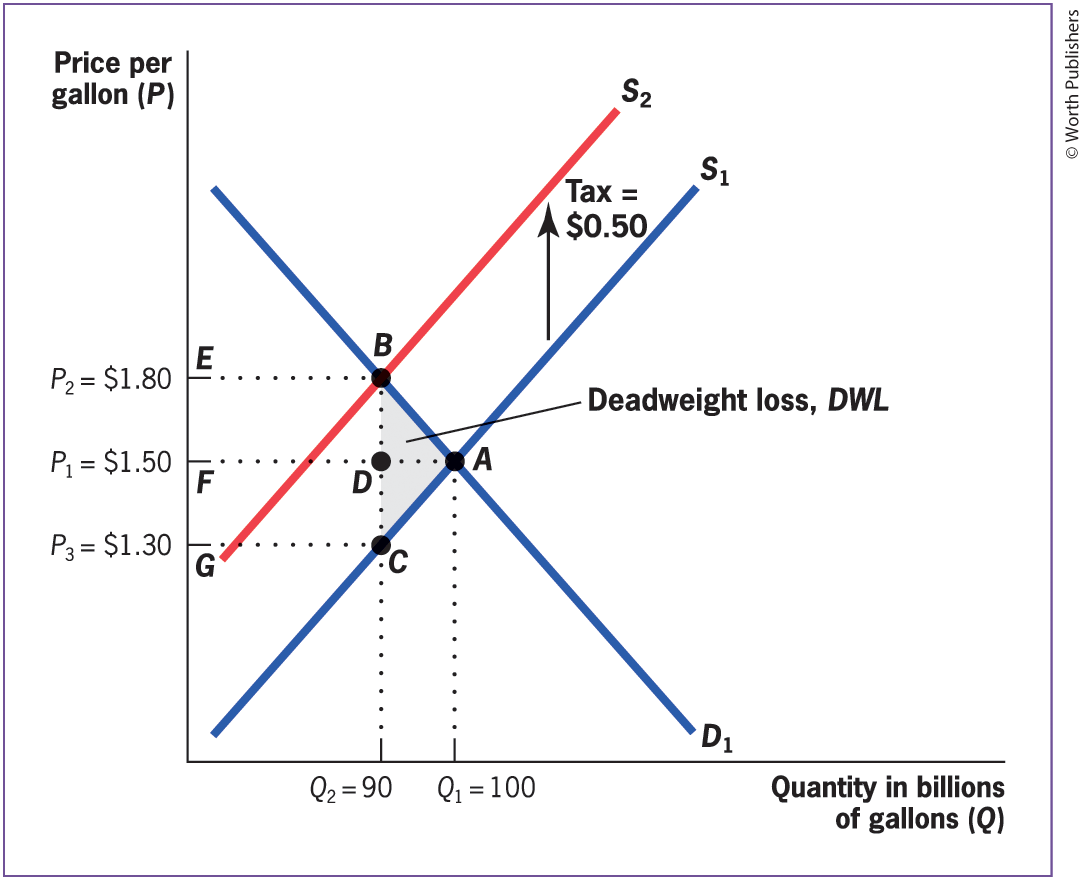
\includegraphics[height=\textheight]{images/figure_17_3.png}
\end{center}
\end{frame}

\begin{frame}
\frametitle{Taxation and Economic Efficiency 3}
\begin{itemize}
  \item Absent taxes: price = social marginal benefit = social marginal cost
  \item The tax drives a wedge between SMB and SMC, preventing mutually beneficial trades from occurring.
  \item The units between 90 and 100 would have generated a consumer and producer surplus.
  \item The forgone surplus from taxation is called the \textbf{deadweight loss (DWL)}.
  \item The size of the DWL depends on elasticities.
\end{itemize}
\end{frame}

\begin{frame}
\frametitle{Elasticities Determine Tax Inefficiency 1}
\begin{itemize}
  \item The deadweight loss of a given tax is smaller when the demand curve is less elastic than when it is more elastic.
\end{itemize}
\begin{center}
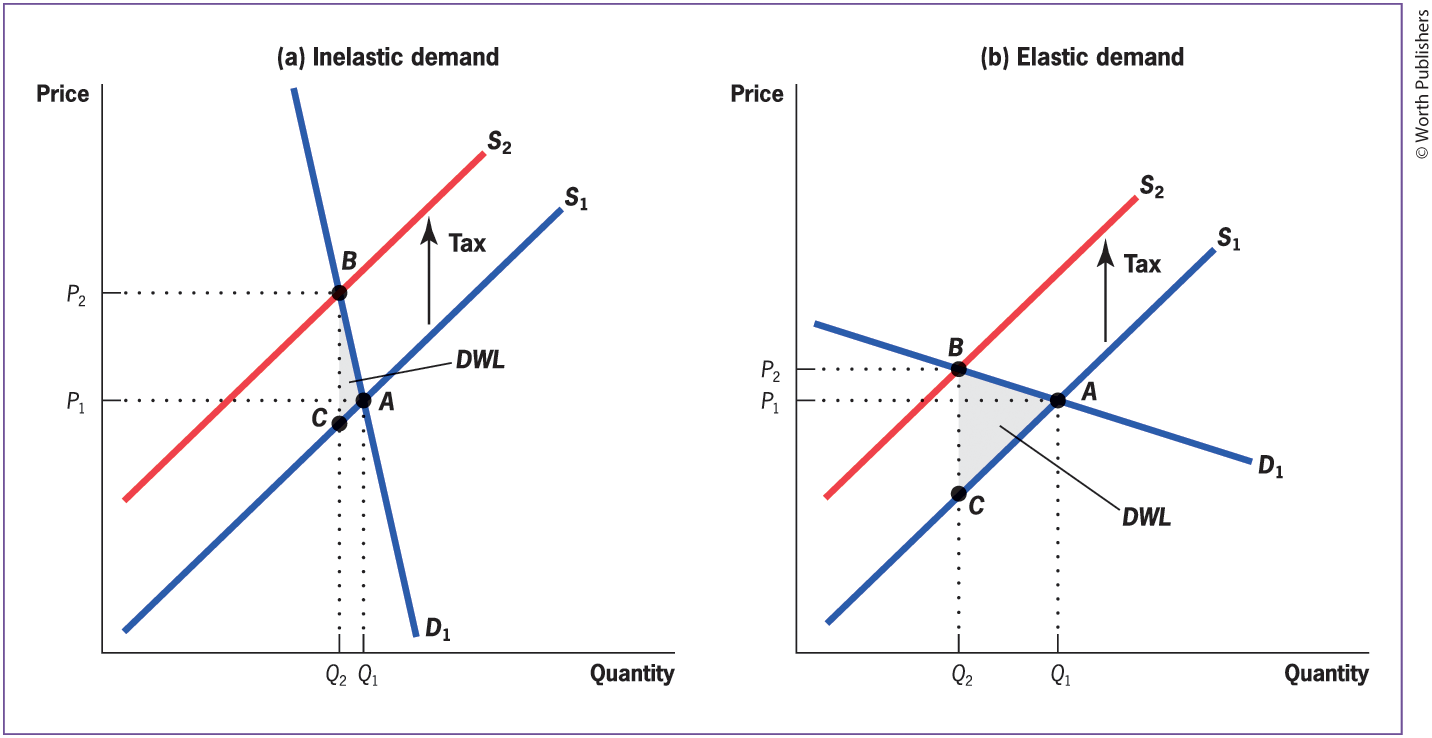
\includegraphics[width=0.9\textwidth]{images/figure_19_3.png}
\end{center}
\end{frame}

\begin{frame}
\frametitle{Elasticities Determine Tax Inefficiency 2}
\begin{itemize}
  \item Deadweight loss is caused by individuals and firms making inefficient consumption and production choices in order to avoid taxation.
  \item The inefficiency of any tax is determined by the extent to which consumers and producers change their behavior to avoid the tax.
  \item The more elastic is demand or supply, the larger the DWL.
\end{itemize}
\end{frame}

\subsection{Empirical Evidence: The Window Tax}

\begin{frame}
\frametitle{Empirical Evidence: The Window Tax 1}
\begin{itemize}
  \item In 1696, English King William III needed money to finance an ongoing war with France.
  \item To raise this revenue, the king imposed a new tax based on the number of windows in a home, which was an indicator of a home's value.
  \item More valuable homes would have more windows and therefore be taxed more highly.
  \item The problem was that individuals could minimize their tax by boarding up or otherwise removing windows.
  \item This rendered the tax a less efficient measure of home value and created a deadweight loss.
\end{itemize}
\end{frame}

\begin{frame}
\frametitle{Empirical Evidence: The Window Tax 2}
\begin{itemize}
  \item Oates and Schwab (2015) presented a straightforward test for whether this was the case: they looked at whether the number of windows responded to ``notches'' in the tax schedule.
  \item From 1747 to 1757:
  \begin{itemize}
    \item No tax if the house had fewer than 10 windows
    \item 6 pence per window for 10 to 14 windows
    \item 9 pence per window if there were 15 to 19 windows
    \item 1 shilling (12 pence) per window for 20 windows or more
  \end{itemize}
  \item The marginal tax rate jumped enormously on building the 10th, 15th, or 20th window.
\end{itemize}
\end{frame}

\begin{frame}
\frametitle{Empirical Evidence: The Window Tax 3}
\begin{itemize}
  \item There are obvious spikes at 9, 14, and 19 windows, exactly what we would predict from the effects of this tax.
\end{itemize}
\begin{center}
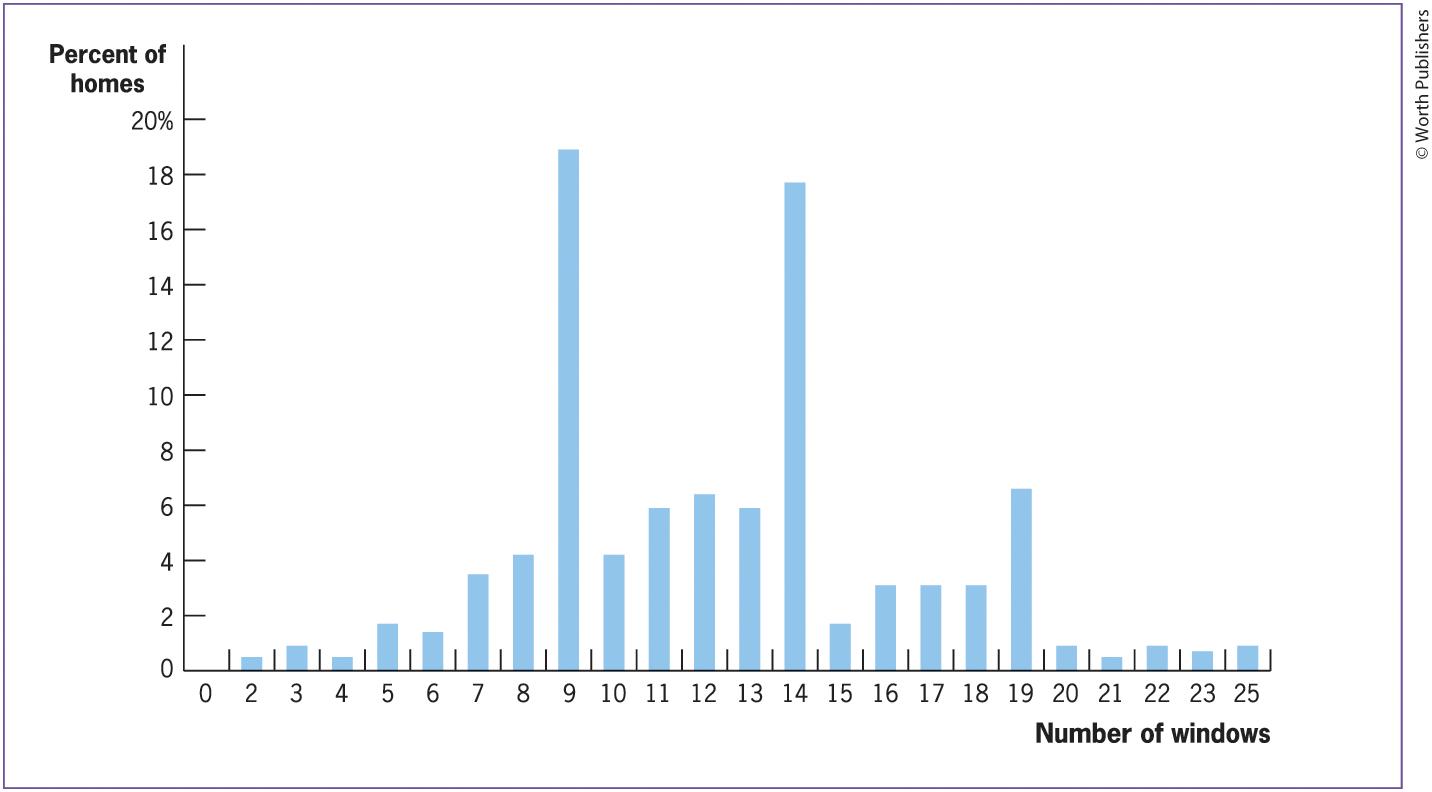
\includegraphics[width=0.85\textwidth]{images/figure_23_3.png}
\end{center}
\end{frame}

\begin{frame}
\frametitle{Empirical Evidence: The Window Tax 4}
\begin{itemize}
  \item One could argue that perhaps there was some British custom or some other reason for having 9, 14, or 19 windows in a house.
  \item Oates and Schwab address this point by using the fact that in 1761, the government added a provision that houses with 8 or 9 windows would pay 1 shilling per window.
  \item This means that after 1761, there was suddenly an incentive to keep the number of windows to 7 or fewer.
  \item This is exactly what happened.
\end{itemize}
\end{frame}

\begin{frame}
\frametitle{Empirical Evidence: The Window Tax 5}
\begin{center}
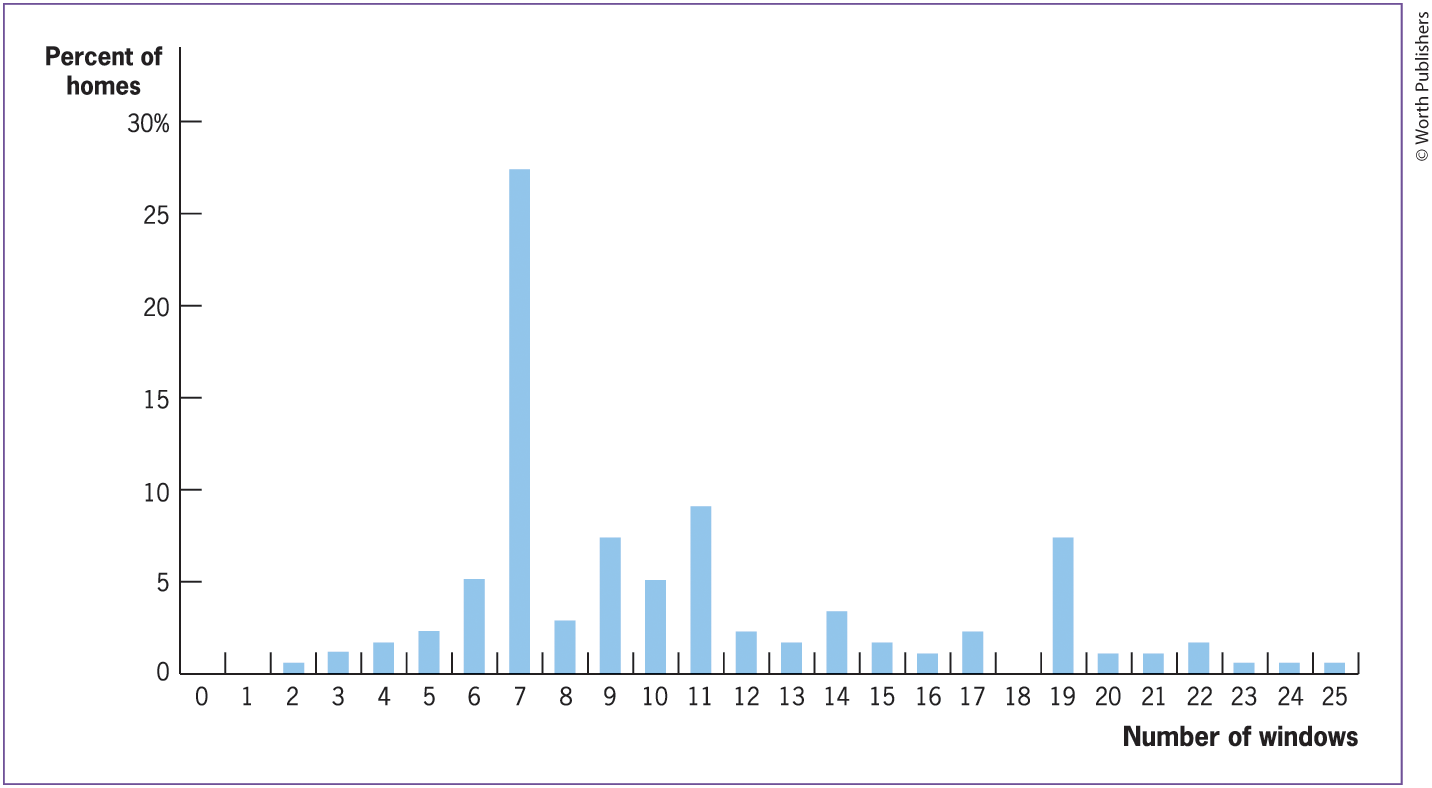
\includegraphics[width=0.95\textwidth]{images/figure_25_3.png}
\end{center}
\end{frame}

\subsection{Progressive Systems}

\begin{frame}
\frametitle{Progressive Tax Systems Can Be Less Efficient 1}
\begin{itemize}
  \item Because the DWL of a tax rises with $\tau^{2}$, progressive tax systems can create larger deadweight losses than proportional systems.
  \item Example:
  \begin{itemize}
    \item Suppose there are two people, one with a wage of \$10 per hour and one with a wage of \$20 per hour.
    \item For both, a 10\% rise in wages causes them to supply 10\% more labor (elasticity of labor supply is 1 for both).
    \item Elasticity of labor demand is also 1.
  \end{itemize}
\end{itemize}
\end{frame}

\begin{frame}
\frametitle{Progressive Tax Systems Can Be Less Efficient 2}
\begin{itemize}
  \item Why is the deadweight loss larger for the higher wage worker, despite the same reduction in hours worked?
  \item In a competitive labor market, the wage equals the marginal product of labor, so the high-wage worker has a higher marginal product of labor.
  \item Society loses twice as much when the high-wage worker reduces her hours than when the low-wage worker reduces her hours.
\end{itemize}
\end{frame}

\begin{frame}
\frametitle{Progressive Tax Systems Can Be Less Efficient 3}
\begin{itemize}
  \item Equal tax on the low-wage worker and the high-wage worker results in deadweight losses shown by triangles BAC and EDF.
\end{itemize}
\begin{center}
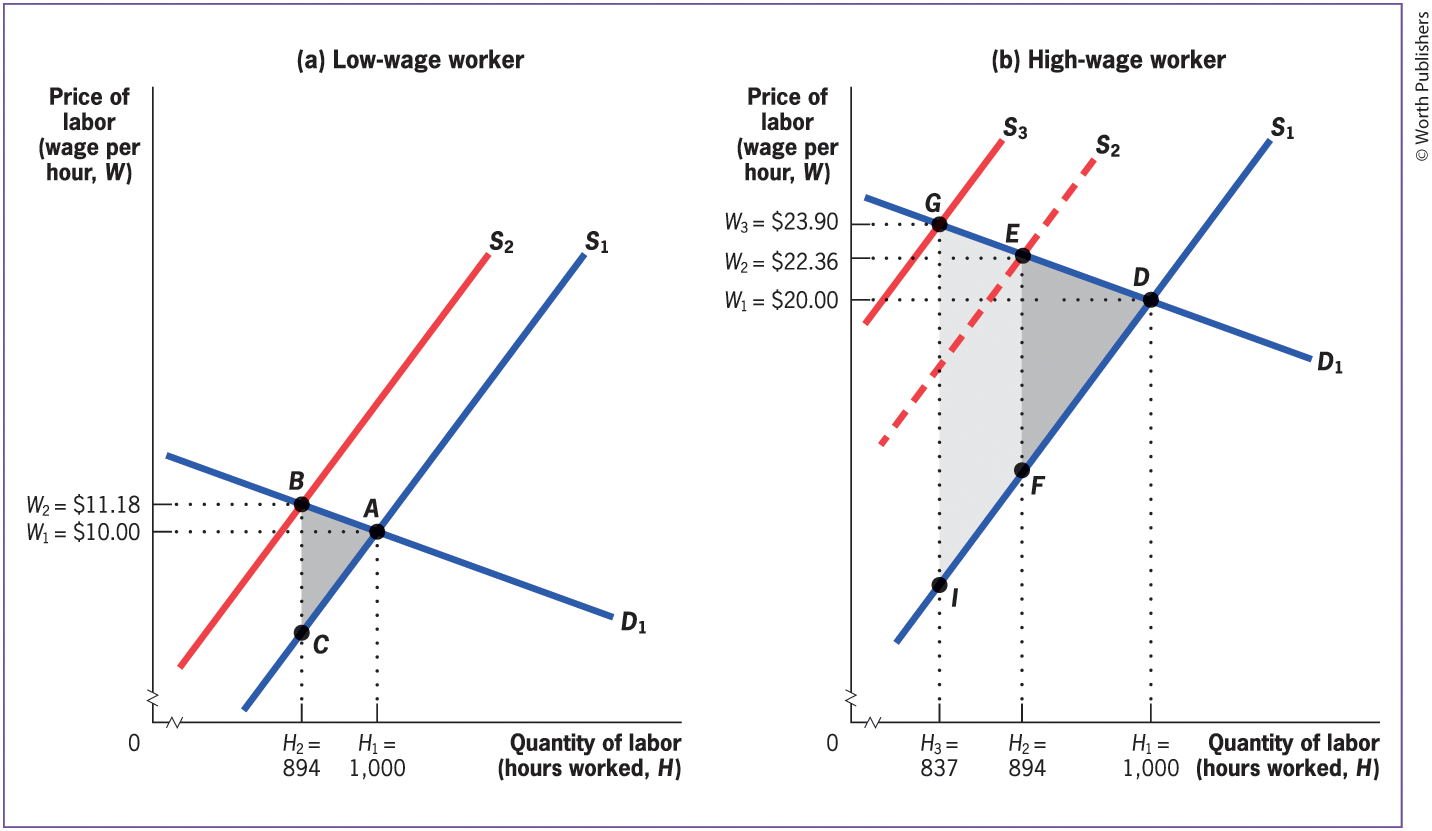
\includegraphics[width=0.83\textwidth]{images/figure_29_3.png}
\end{center}
\end{frame}

\begin{frame}
\frametitle{Progressive Tax Systems Can Be Less Efficient 4}
\begin{itemize}
  \item No tax on low-wage worker (no DWL) and high tax for high-wage worker: DWL for the high-wage worker increases by the trapezoid GEFI.
\end{itemize}
\begin{center}
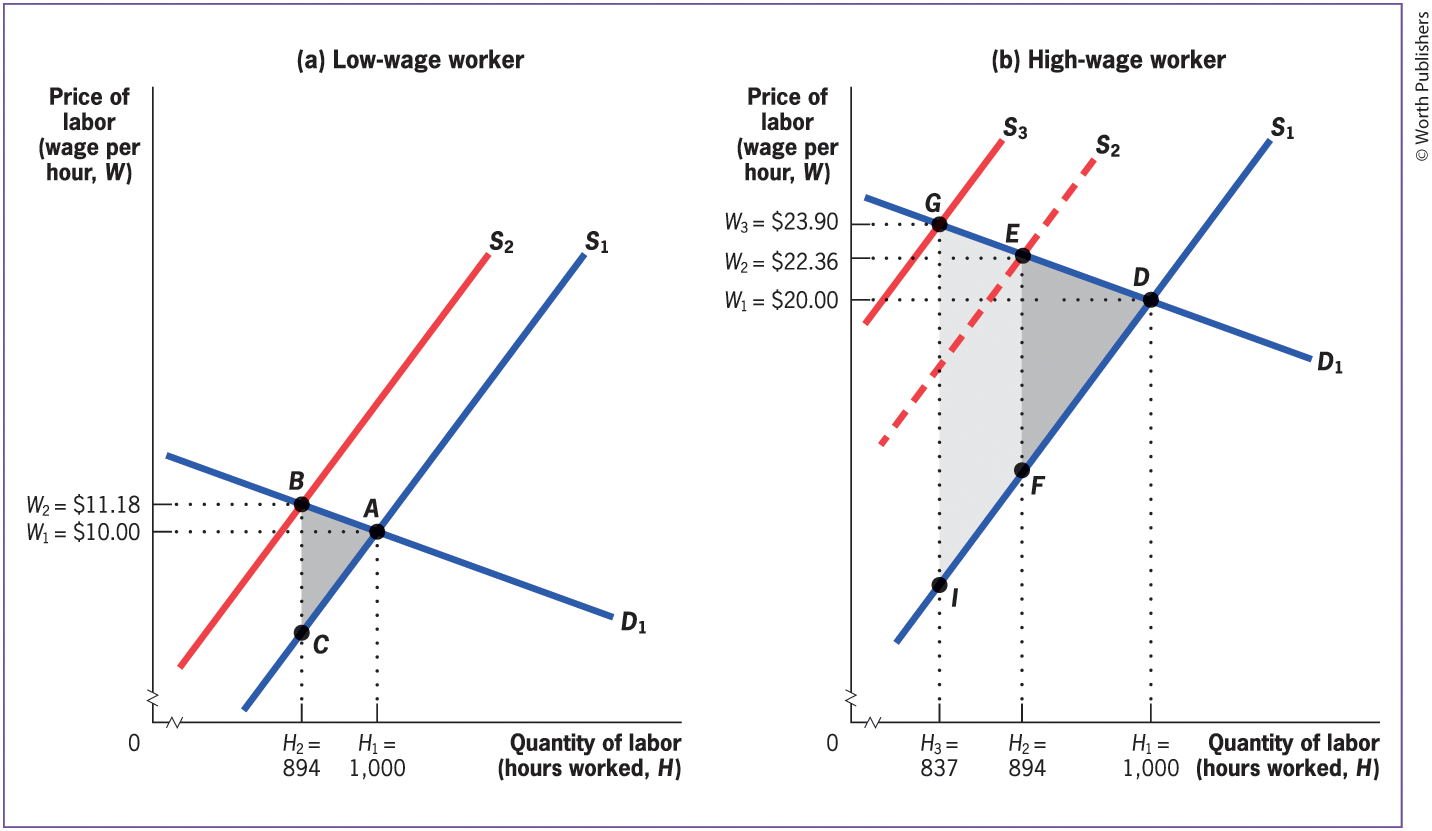
\includegraphics[width=0.83\textwidth]{images/figure_30_3.png}
\end{center}
\end{frame}

\begin{frame}
\frametitle{Progressive Tax Systems Can Be Less Efficient 5}
\begin{center}
\small
\begin{tabular}{llllllll}
\toprule
 & \multicolumn{2}{c}{Tax Schedule} & \multicolumn{2}{c}{Low-Wage Worker} & \multicolumn{2}{c}{High-Wage Worker} & \\
\cmidrule(lr){2-3} \cmidrule(lr){4-5} \cmidrule(lr){6-7}
 & Tax Below & Tax Above &  Hours & DWL & Hours & DWL & Total \\
 & \$10,000 & \$10,000 & Supply & of Tax & Supply & of Tax & DWL \\
\midrule
No tax & 0\% & 0\% & 1,000 & 0 & 1,000 & 0 & 0 \\
Proportional & 20\% & 20\% & 894 & \$115.71 & 894 &\$231.42 & \$347.13 \\
Progressive & 0\% & 60\% & 1,000 & 0 & 837 & \$566.75 & \$566.75 \\
\bottomrule
\end{tabular}
\end{center}
\begin{itemize}
  \item The deadweight loss is larger for the higher-wage worker, despite the same reduction in hours worked.
\end{itemize}
\end{frame}

\subsection{Optimal Income Taxation}

\begin{frame}
\frametitle{Optimal Income Taxes}
\begin{itemize}
  \item Most tax revenue in the United States and other developed countries is from income taxes.
  \item \textbf{Optimal income taxation}: Choosing the tax rates across income groups to maximize social welfare subject to a government revenue requirement.
  \item Social welfare function guides the trade-off between progressivity and efficiency.
\end{itemize}
\end{frame}

\begin{frame}
\frametitle{A Simple Example 1}
\begin{enumerate}
  \item Everyone has the same utility function:
  \begin{equation*}
    U_{1} = U_{2} = \ldots
  \end{equation*}
  \item These utility functions exhibit diminishing marginal utility of income.
  \item Total income in society is fixed. Not determined by individual choices that might respond to taxes.
  \item Society maximizes the sum of utilities of all individuals.
  \begin{equation*}
    W = U_{1} + U_{2} + \ldots
  \end{equation*}
\end{enumerate}
\end{frame}

\begin{frame}
\frametitle{A Simple Example 2}
\begin{itemize}
  \item Under these assumptions:
    \item The optimal income tax system is one that leaves everyone with the same level of post-tax income.
    \item People with below average incomes would receive transfers to increase their incomes to average.
    \item The marginal tax rate under this system is 100\%.
  \item If income responds to taxes, the optimal marginal tax rate is lower.
\end{itemize}
\end{frame}

\begin{frame}
\frametitle{General Model with Behavioral Effects 1}
\begin{itemize}
  \item With behavioral effects, taxes reduce hours worked. 
  \item At high tax rates, tax revenue falls with the tax rate; no one works under a 100\% tax rate. 
  \item The optimal tax system trades off the efficiency cost of taxation against the benefits of redistribution.
  \item The rule is to set the income for group $i$ such that
  \begin{equation*}
     \frac{MU_{i}}{MR_{i}} = \lambda
  \end{equation*}
  \item $MU_{i}$ is the marginal utility of income for group $i$, $MR_{i}$ is the marginal revenue from taxing group $i$, and $\lambda$ is the value of government revenue.
\end{itemize}
\end{frame}

\begin{frame}
\frametitle{The Laffer Curve}
\begin{itemize}
  \item From 0 to $\tau^*$, tax revenues rise. With tax rates above $\tau^*$, tax revenues fall.
\end{itemize}
\begin{center}
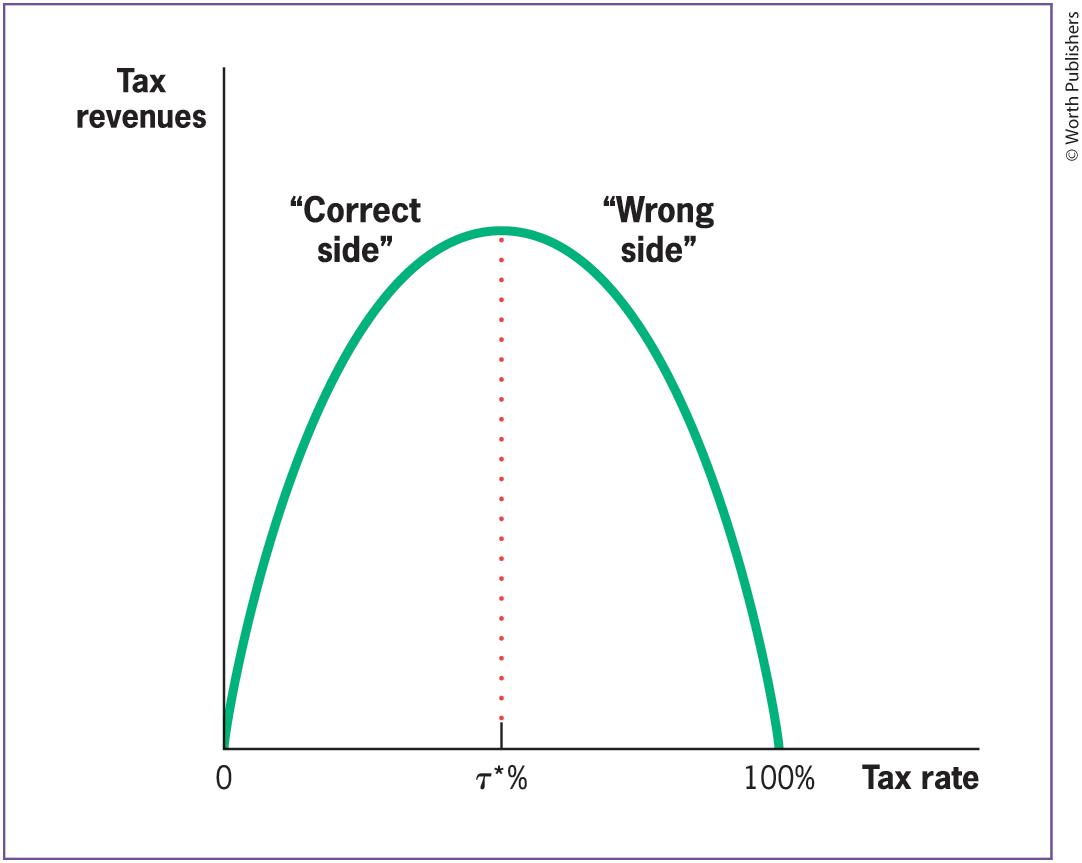
\includegraphics[height=\textheight]{images/figure_36_3.png}
\end{center}
\end{frame}

\begin{frame}
\frametitle{General Model with Behavioral Effects 2}
\begin{itemize}
  \item Optimal income taxation balances:
  \item \textbf{Vertical equity}: Social welfare is maximized when those who have a high level of consumption and thus a low marginal utility of consumption are taxed more heavily and when those who have a low level of consumption and thus a high marginal utility of consumption are taxed less heavily.
  \item \textbf{Behavioral responses}: As taxes rise on any one group, individuals in that group may respond by earning less income.
\end{itemize}
\end{frame}

\begin{frame}
\frametitle{An Example: Optimal Income Taxes with Two Types}
\begin{itemize}
  \item Ratio of MU to MR rises as tax rates rise for any taxpayer.
  \item Ratio for Dr. H < ratio for Dr. L. Optimal income tax rates equate this ratio across taxpayers. $\Rightarrow$ optimal rates: 10\% for Dr. L and 20\% for Dr. H.
\end{itemize}
\begin{center}
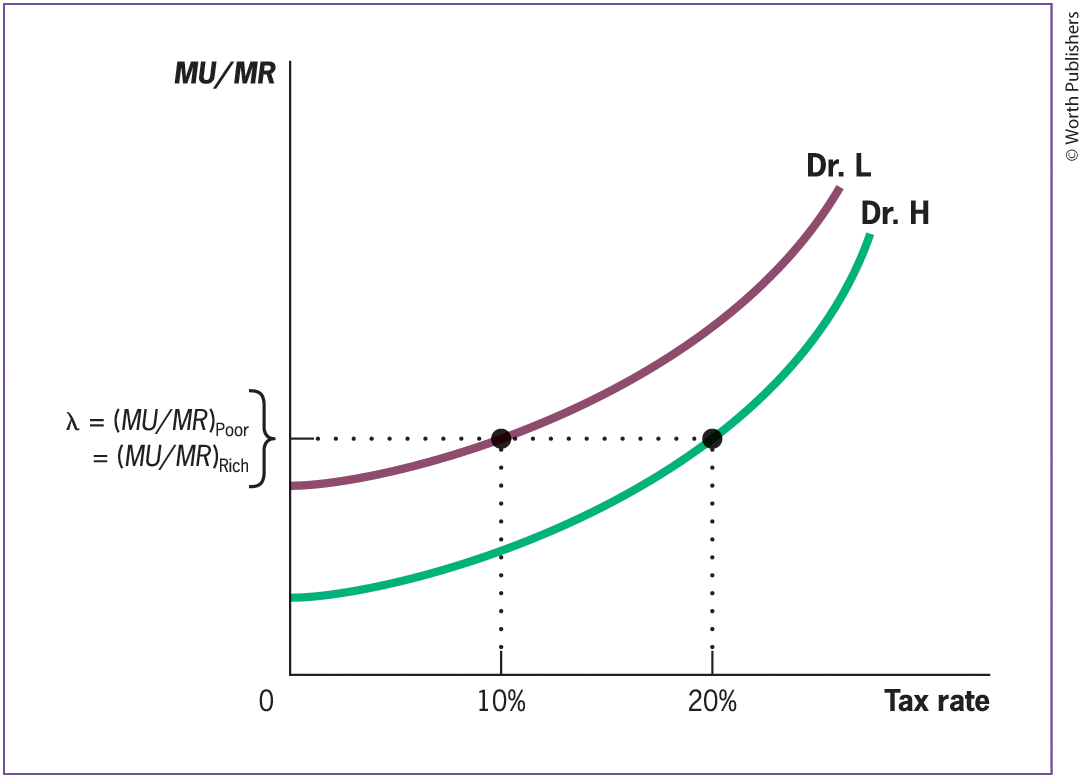
\includegraphics[width=0.64\textwidth]{images/figure_38_3.png}
\end{center}
\end{frame}

\begin{frame}
\frametitle{Conclusion}
\begin{itemize}
  \item The fundamental issue in designing tax policy is the equity-efficiency trade-off.
  \item Tax efficiency comes down to two key principles:
  \begin{itemize}
    \item The more elastically supplied or demanded the good, the larger the deadweight loss from the tax.
    \item The higher the tax rate, the larger the incremental deadweight loss of taxation.
  \end{itemize}
\end{itemize}
\end{frame}

\section{Income Shares and the Elasticity of Taxable Income}

\begin{frame}
  \frametitle{Income Shares and the ETI}
  \begin{itemize}
    \item The elasticity of taxable income (ETI) is the key statistic we need to assess the deadweight loss of the income tax.
    \item The income shares approach (Saez, 2004) to estimating the ETI involves looking at how the \textit{share} of total income earned by a group experiencing a tax cut/increase changes in response to changes in the tax rate they face.
    \item Implicitly a diff in diff with the rest of the population as the control group (to control for macro trends)
    \item Big advantage: We can do this using aggregate statistics!
  \end{itemize}
  \begin{align*}
    e & = \frac{\log(p_{t_{1}}) - \log(p_{t_{0}})}{\log(1 - \tau_{p,t_{1}}) - \log(1 - \tau_{p,t_{0}})} \\
    \log(p_{t}) & = \alpha + e \cdot \log(1 - \tau_{p,t}) + \varepsilon_{t}
  \end{align*}
\end{frame}


\begin{frame}
  \frametitle{Saez (2004): Top 1\% Income Share}
  \begin{center}
    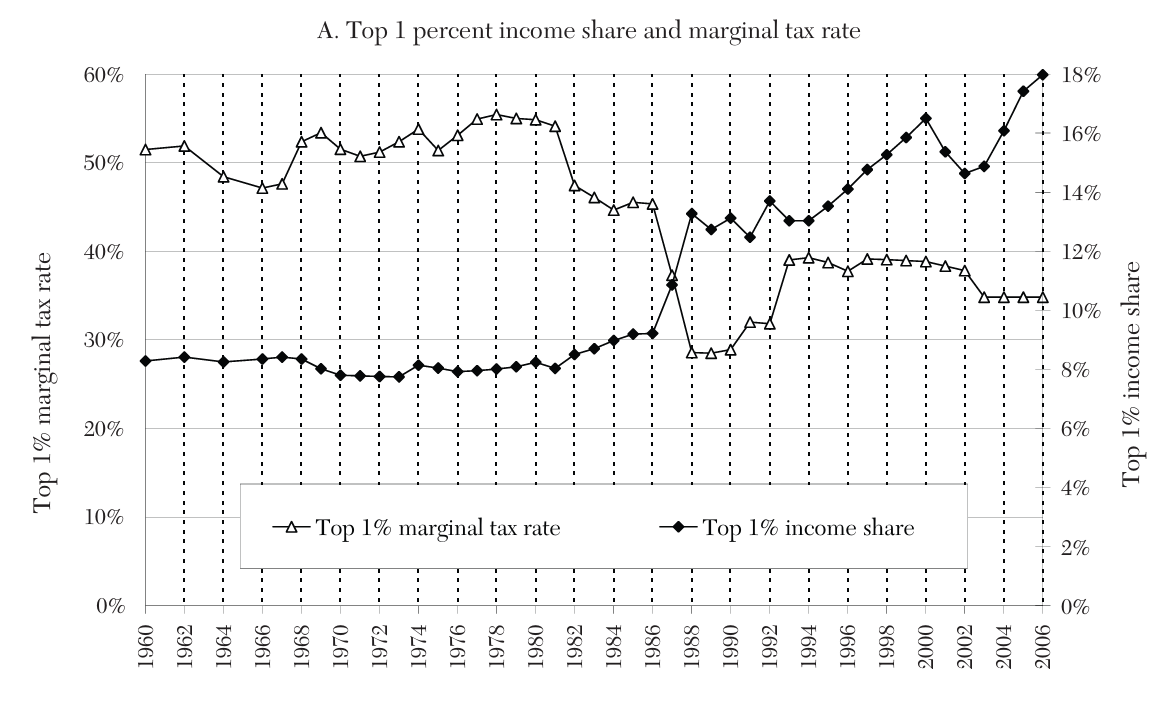
\includegraphics[width=0.91\textwidth]{images/Saez2004_top1percent.png}
  \end{center}
\end{frame}


\begin{frame}
  \frametitle{Saez (2004): Next 9\% Income Share}
  \begin{center}
    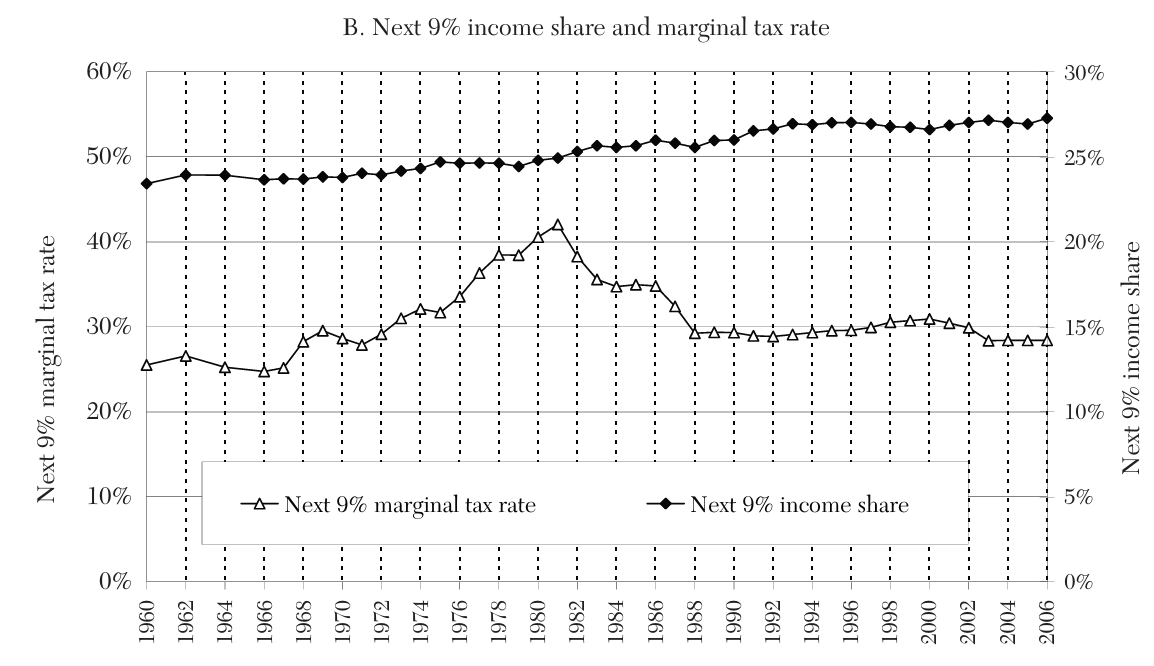
\includegraphics[width=0.94\textwidth]{images/Saez2004_next9percent.png}
  \end{center}
\end{frame}


\begin{frame}
  \frametitle{Saez (2004): Elasticities}
  \begin{center}
    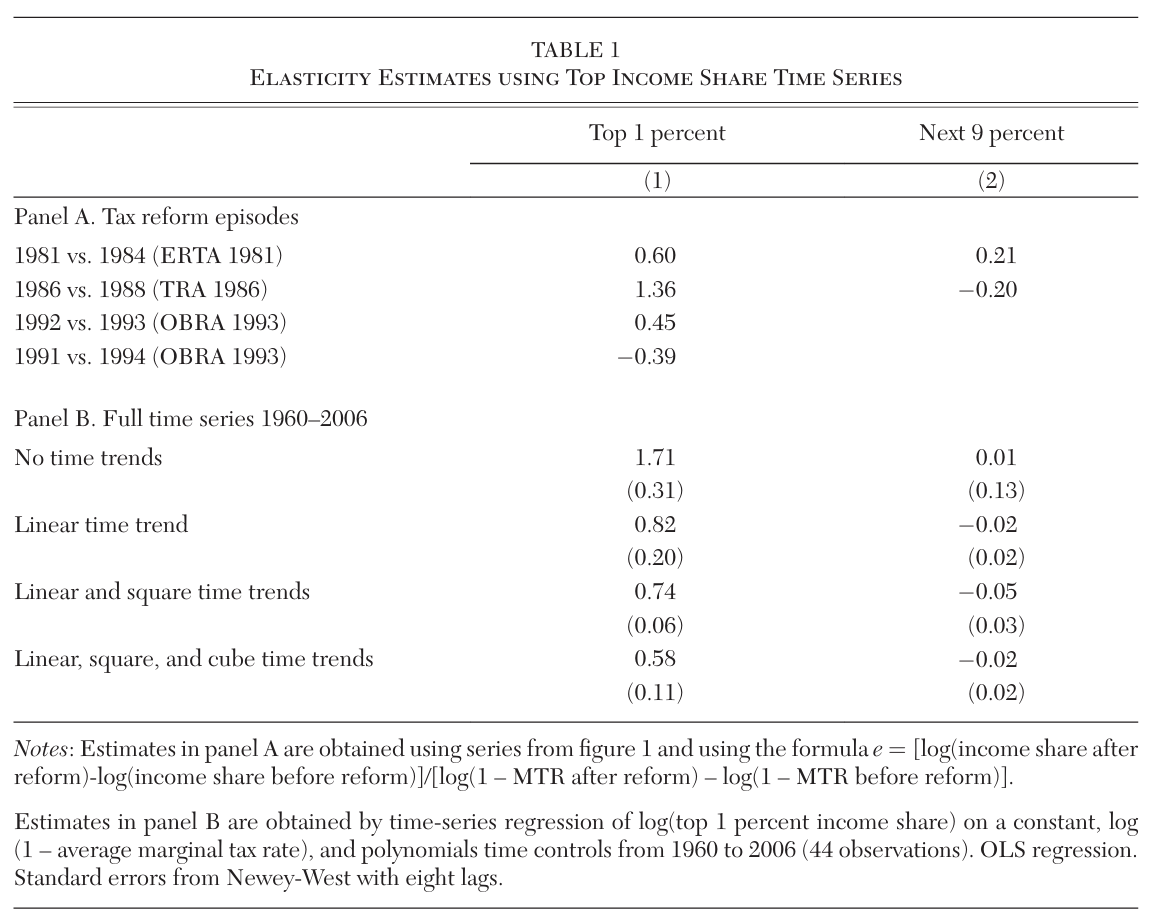
\includegraphics[height=0.99\textheight]{images/Saez2004_elasticities.png}
  \end{center}
\end{frame}

\section{Over to You}

\begin{frame}
\frametitle{The Tax Cuts and Jobs Act of 2017}
\begin{itemize}
  \item The Tax Cuts and Jobs Act of 2017 was a major overhaul of the U.S. tax code that included significant changes to individual income tax rates, corporate tax rates, and various deductions and credits.
  \item The act reduced the top marginal tax rate from 39.6\% to 37\% and lowered tax rates for other income brackets as well.
  \item It also increased the standard deduction and eliminated personal exemptions, among other changes.
  \item Let's use the income shares approach to estimate the elasticity of taxable income in response to the tax cuts for different income groups and different types of taxpayers.
  \begin{enumerate}
    \item Top earners vs middle class
    \item Married vs single
  \end{enumerate}
\end{itemize}
\end{frame}

\begin{frame}
  \frametitle{The Tax Cuts and Jobs Act of 2017: MTRs}
  \begin{center}
    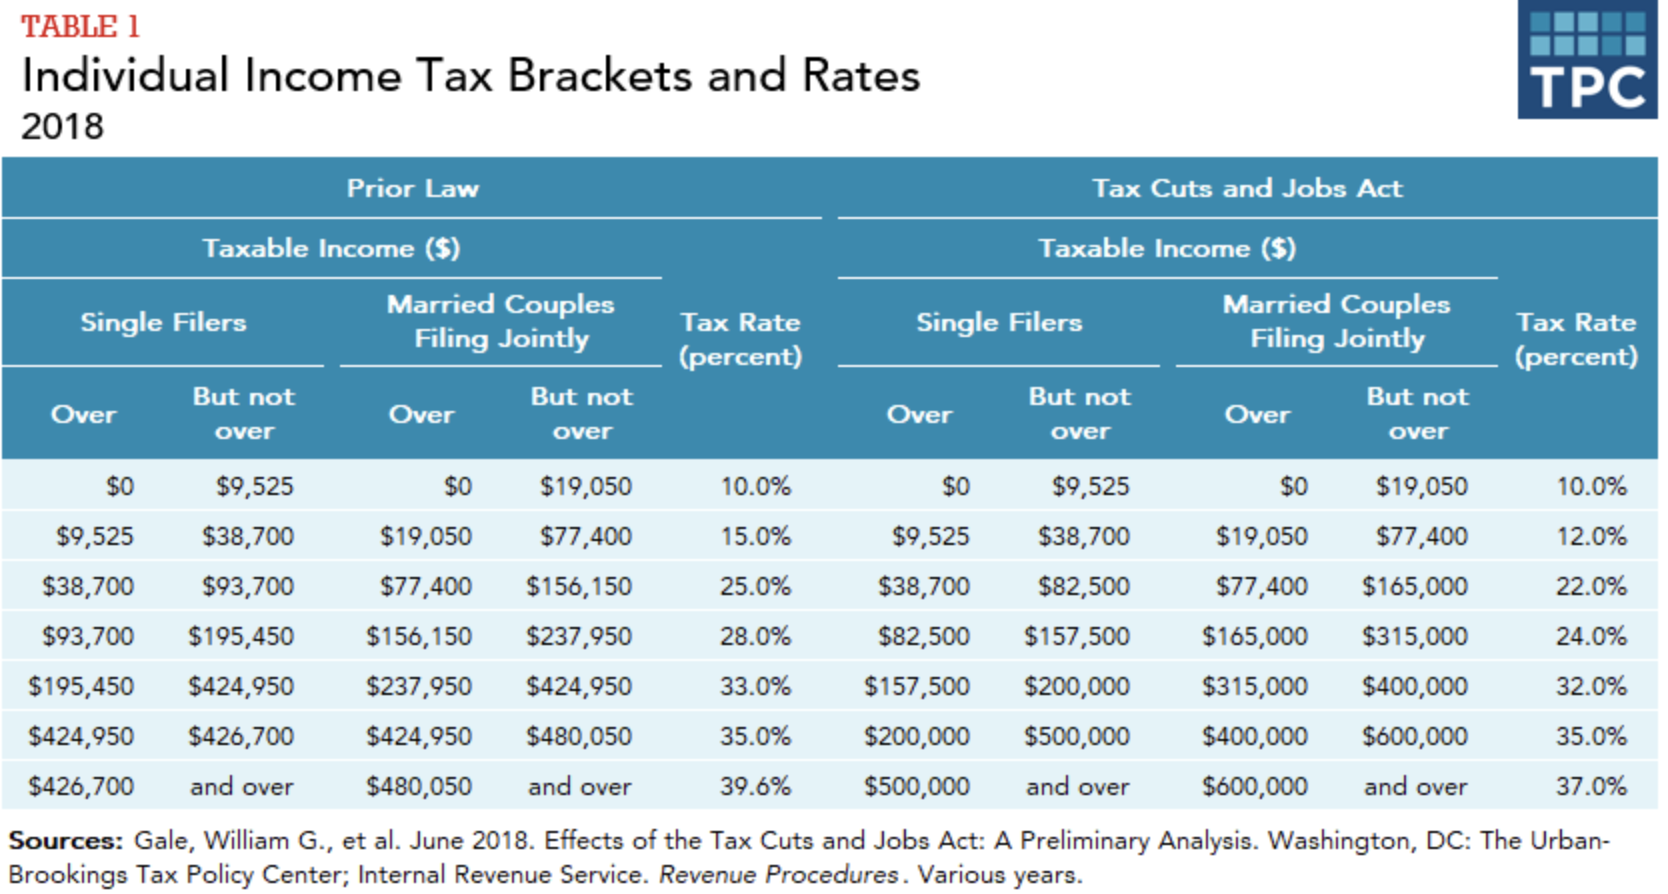
\includegraphics[width=0.95\textwidth]{images/TCJA_MTRs.png}
  \end{center}
\end{frame}

\begin{frame}
  \frametitle{Steps}
  \begin{enumerate}
    \item Three groups: 
    \begin{enumerate}
      \item Top bracket \& married
      \item top bracket \& single
      \item middle class (28\% -> 24\%) \& single
    \end{enumerate}
    \item Grab the SOI data \href{https://www.irs.gov/statistics/soi-tax-stats-individual-statistical-tables-by-size-of-adjusted-gross-income}{\url{https://www.irs.gov/statistics/soi-tax-stats-individual-statistical-tables-by-size-of-adjusted-gross-income}}
    \item Do shares analysis for your treated group
    \item Do shares analysis for a nearby control group
    \item Let's discuss the elasticities we find!
  \end{enumerate}
\end{frame}

\end{document}
